\documentclass[a4paper,12pt]{article}
\title{\textbf{Anleitung für ZM1000 Nixi Uhr \newline Von Moritz für Mama}}

\usepackage{graphicx}
\usepackage{subcaption}
\usepackage{multirow}
\usepackage{xcolor,colortbl}

\newcommand{\mc}[2]{\multicolumn{#1}{c}{#2}}
\definecolor{Gray}{gray}{0.85}
\definecolor{LightCyan}{rgb}{0.88,1,1}

\newcolumntype{a}{>{\columncolor{Gray}}c}
\newcolumntype{b}{>{\columncolor{white}}c}

\begin{document}
\maketitle

\begin{figure}[h!]
    \centering
    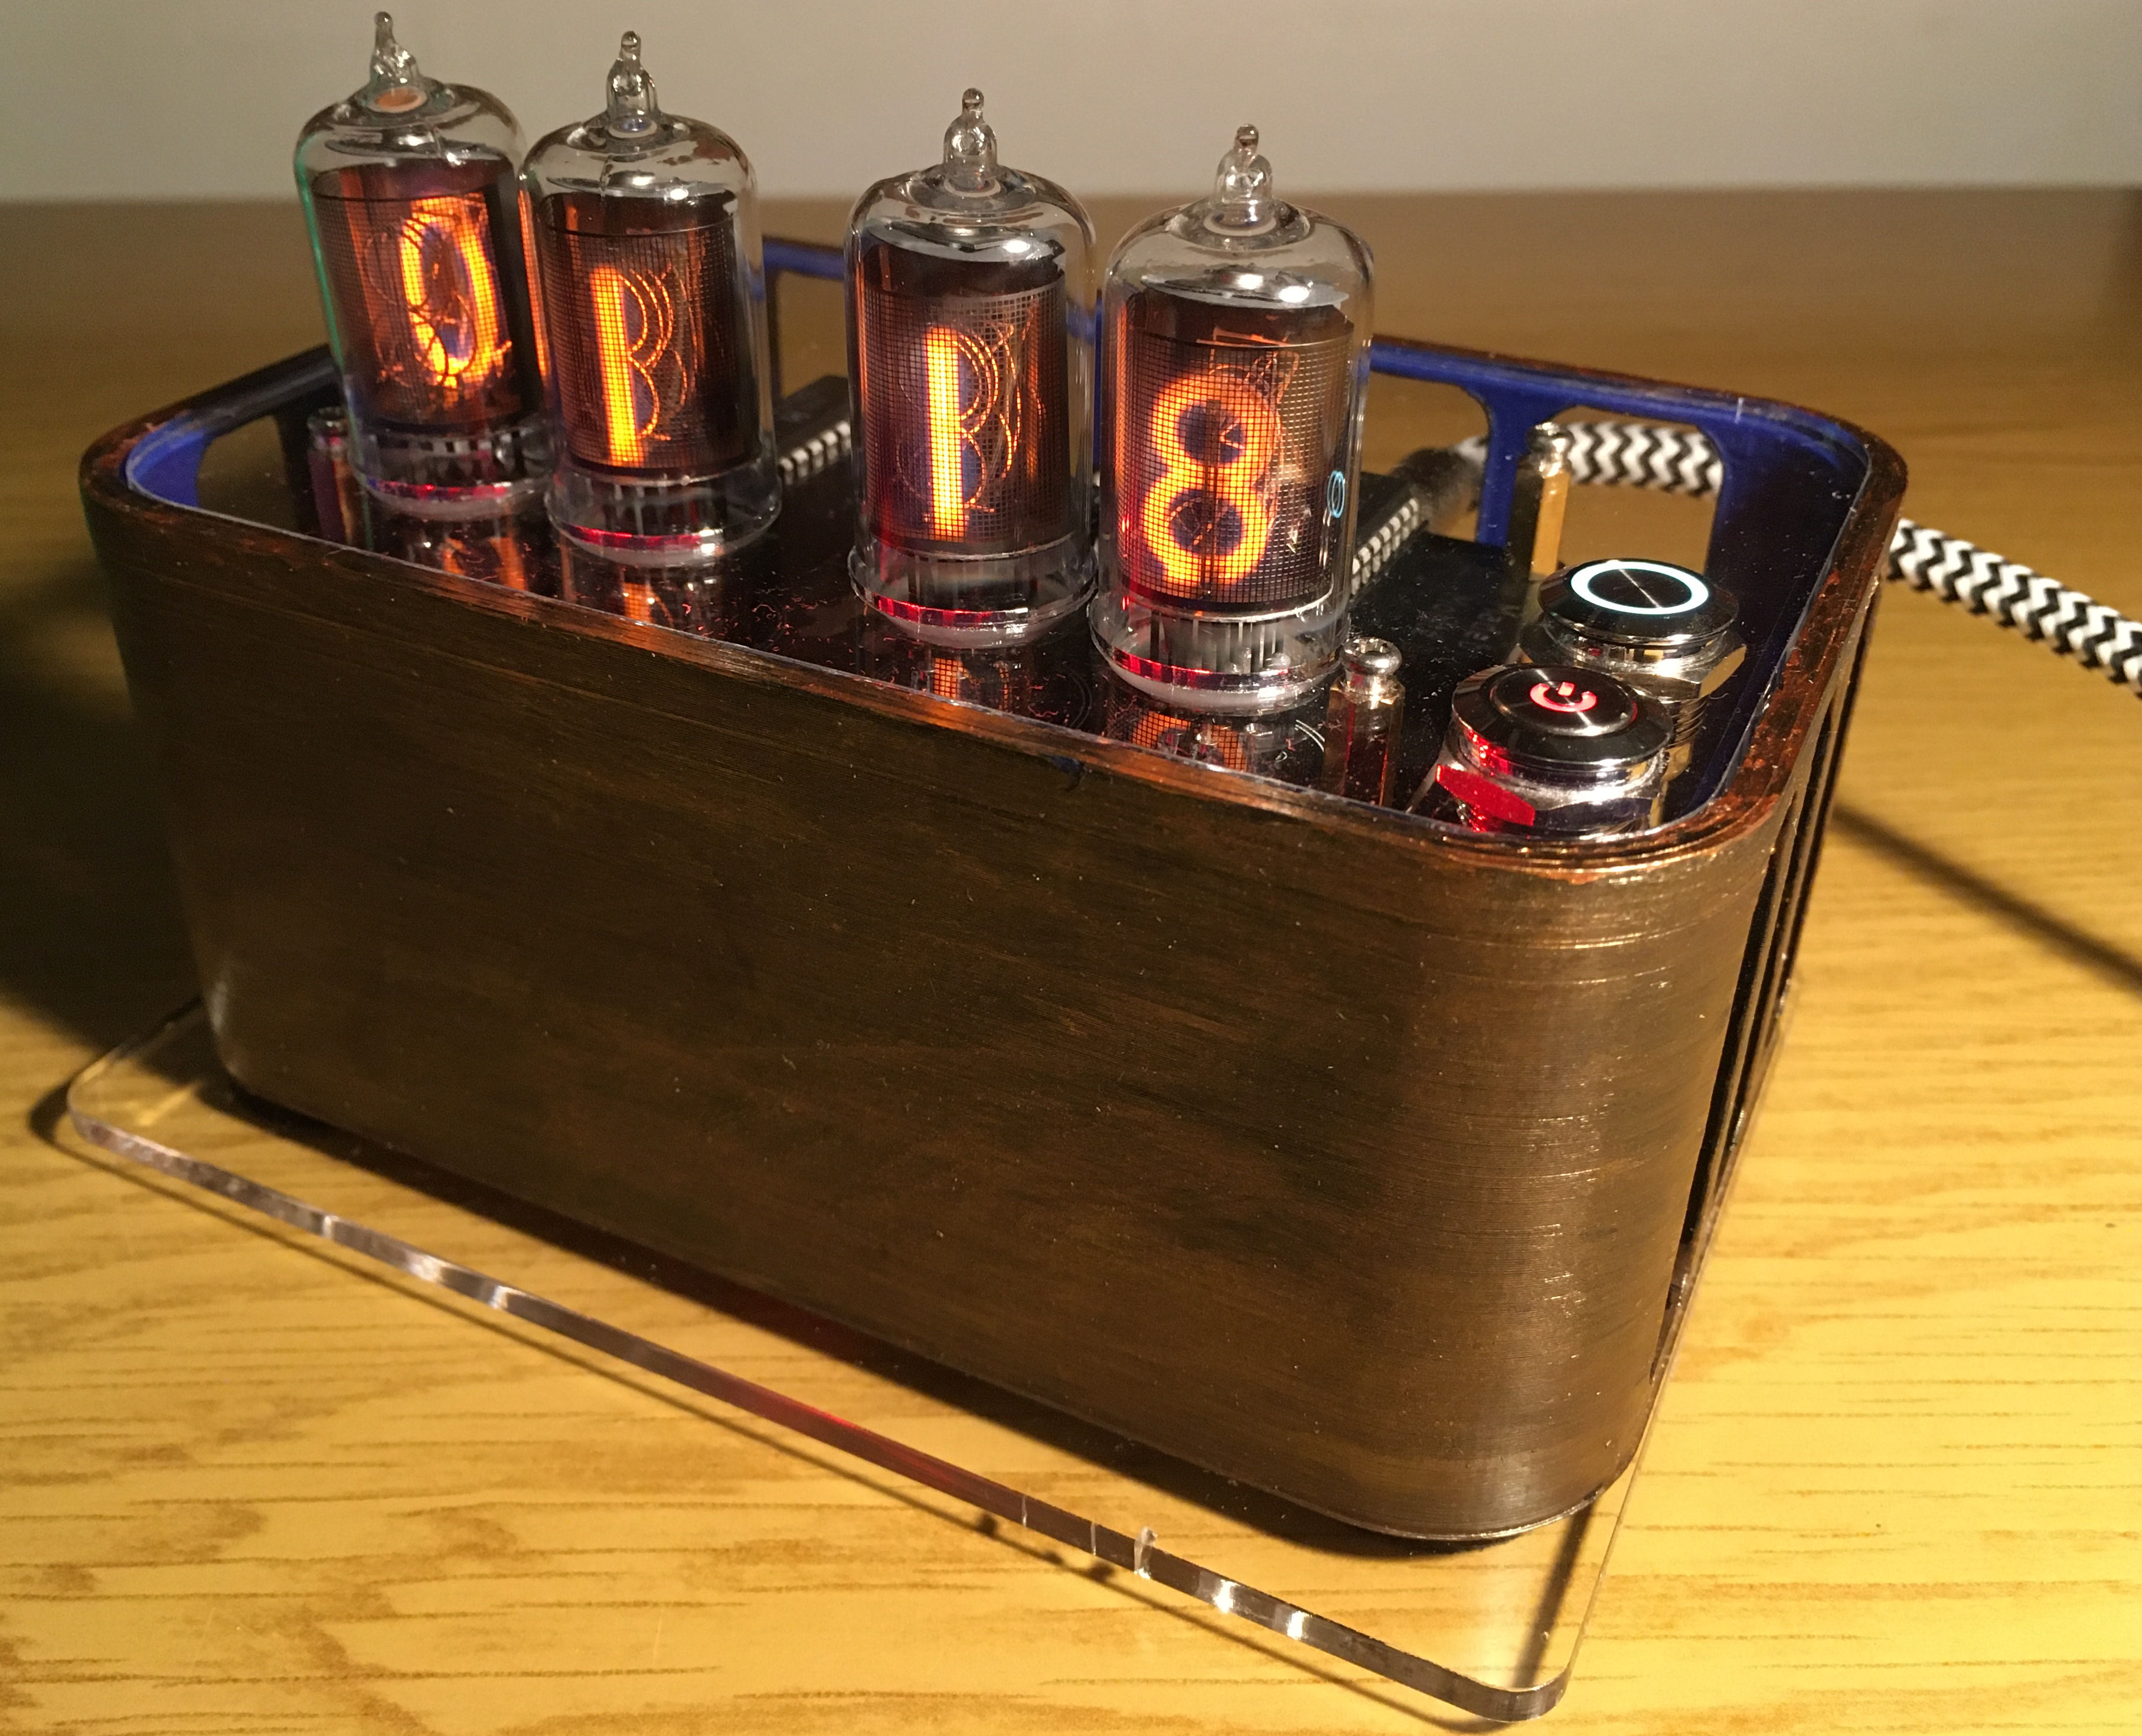
\includegraphics[width=1\textwidth]{Clock.jpg}
\end{figure}



\newpage

\section{Einleitung}

Die Uhr hat einen \textbf{Power Button} und einen \textbf{Funktions Button} beide sind auf der rechten Seite (von vorne gesehen) auf der Uhr zu finden.

\begin{figure}[h!]
    \centering
    \begin{subfigure}[b]{0.1\textwidth}
        
\includegraphics[width=\textwidth]{Power_BTN.png}
    \end{subfigure}
    ~ %add desired spacing between images, e. g. ~, \quad, \qquad, \hfill etc. 
      %(or a blank line to force the subfigure onto a new line)
    \begin{subfigure}[b]{0.1\textwidth}
        
\includegraphics[width=\textwidth]{Push_BTN.png}
    \end{subfigure}
\end{figure}

\section{Funktion}

\begin{center}
\begin{tabular}[h]{|p{1.3cm}|p{3cm}|p{3cm}|p{6cm}|}
    \hline
    \rowcolor{LightCyan}
    \multirow{2}{*}{\textbf{Knopf}} & \multirow{2}{*}{\textbf{Funktion}} & \multirow{2}{*}{\textbf{Druckdauer}} & \multirow{2}{*}{\textbf{Uhrzeit anzeigen}} \\
    &  &  & \\
    \hline
    \multirow{3}{*}{
\includegraphics[\textwidth]{Power_BTN.png}} & \multirow{3}{*}{Standby} & \multirow{3}{*}{kurz} & \multirow{3}{*}{Erneutes drücken} \\
     &  &  & \\
     &  &  & \\
    \hline
    \multirow{3}{*}{
\includegraphics[\textwidth]{Push_BTN.png}} & \multirow{3}{*}{Temp. \& Luftf.} & \multirow{3}{*}{kurz} & \multirow{3}{*}{Automatisches Ende} \\
     &  &  & \\
     &  &  & \\
    \hline
    \multirow{3}{*}{
\includegraphics[\textwidth]{Push_BTN.png}} & \multirow{3}{*}{Stoppuhr} & \multirow{3}{*}{lang} & \multirow{3}{*}{Power Button drücken} \\
     &  &  & \\
     &  &  & \\
    \hline
\end{tabular}
\end{center}

\section{Internetverbindung}

Ist die Verbindung zum Internet gegeben wird bei der Anzeige der Temperatur und Luftfeuchtigkeit bei den letzten beiden Ziffern die Aussentemperatur angezeigt.
  
\end{document}